\documentclass[12pt]{article}

\usepackage{geometry}
\geometry{margin=1in}
\usepackage{graphicx}
\usepackage[english]{babel}
\usepackage{fancyhdr}
\pagestyle{fancy}
\fancyhf{}
\lhead{Spring 2021 --- PHYS 432 Lab 3}
\rhead{Helen (Yeu) Chen}
\setlength{\parindent}{0cm}
\usepackage{makecell}
\usepackage{amsfonts}
\usepackage{longtable}
\usepackage{amsmath}
\usepackage{amssymb}
\usepackage{amsthm}
\graphicspath{ {./images/} }


\fancyfoot[C]{\thepage}

\begin{document}
\textbf{The Franck-Hertz Experiment}
\bigskip

\textbf{1. \textit{Introduction}}
\smallskip

In this experiment we explore the current vs. voltage plot collected from both the neon and mercury Franck Hertz tube to determine the first excited state energy of both atoms. In the Franck Hertz experiment we vary the voltage across a Franck Hertz tube, which is filled with either Hg or Ne vapor, at a steady rate. Electrons travel from the cathode toward the anode while colliding with atoms along their why. The electron can experience either elastic collision, in which it lost almost no energy, or inelastic collision, in which it gives up almost all its energy to excited the atom. The type of collision that occurs depends on the kinetic energy of the electron, that is, if it has enough energy to cause an excitation. If electron arrives at the grid (positioning in front the anode) with low energy (i.e after experiencing an inelastic collision) then it is filtered out by the grid hence reducing the current recorded at the anode. Since amount of energy gained by an electron depend on the voltage applied, we see the current at the anode changes with the accelerating voltage.

Our experiment is based largely on Rapior, Sengstock and Baev's paper, "New features of the Franck-Hertz experiment". In which, they suggested that total energy gain by an electron at the troughs location of the IV plot follows
\begin{equation}\label{eqn:einstein}
E_n = E_a \frac{\lambda}{L}n^2 + E_a n+c
\end{equation}
where $E_n$ is the energy gain at $n$th trough, $E_a$ is the first excited state of the atom, $\lambda$ is the mean free path of electron, $c$ a constant, and $L$ is the distance between the cathode and the grid. Moreover, the difference of energy follows 
\begin{equation}\label{eqn:einstein}
\Delta E(n) = E_n - E_{n-1} =E_a(1-\frac{\lambda}{L}) + 2E_a\frac{\lambda}{L}n
\end{equation}
Notice that $E_a = \Delta E(\frac{1}{2})$, this will be one of the relation we use to find the first excited state energy $E_a$.
\bigskip

\textbf{2. \textit{Lowest excited state energy $E_a$}}
\smallskip

For Ne, following the method of linear fit to energy difference introduced in the RSB paper, the first excited energy was calculated to be $14.558 \pm 0 \;eV$, while by simply averaging the trough differences, $E_a$ was calculated to be $18.054 \pm 0.505 \;eV$. For Hg, the RSB method gives $E_a = 4.690 \pm 0.063 \; eV$ and the simple averaging gives $E_a = 5.069\pm 0.039 \; eV$. We see that in both cases, the averaging method gives a larger energy than the RSB method. This result is expected and explained in the RSB paper. In short, from equation (2) one can see that the trough differences growths with $n$ and deviates more from $E_a$ as $n$ increases. Hence, averaging the trough differences over estimate the first excited state energy.

If comparing the known first excited state values, where Ne has $E_a = 16.6 \; eV$ and Hg has $E_a = 4.67 \; eV$, we found that our Ne RSB result does not give a good estimate. One possible reason is that on our experiment, we did not vary the accelerating voltage to a very high value, hence we only recorded three troughs for Ne. This means when fitting the energy difference, there are only two data points available. Hence any small impreciseness in recording the trough locations, results in a less accurate first excited state energy. In the RSB paper, they vary the voltage up to $80+$ volts, and got a closer value of $16.5\pm0.2\; eV$.
\bigskip

\textbf{3. \textit{Light band formation in neon Franck Hertz tube}}
\smallskip

As the accelerating voltage sweep through a range from $0V$ to $70V$, there are different number of orange light bands forming between the cathode and the grid. This orange light corresponds to the energy transition between the 3s-3p levels (after the atom being excited to 3p state, its energy drops down in steps where 3p-3s is the first step). One can’t see the transition from the 3s-ground state because this transition does not fall into the range of visible light. Roughly at each trough, a new light band is formed, while the older light bands move towards the cathode as the voltage increases. This agrees with our model since it stated that at the first trough, the electron gained enough energy to make one inelastic collision, and at the second trough, enough energy for two collisions and so on. The number of bands corresponds to how many inelastic collisions has happened as electrons travel from cathode to the grid, so we see 1 band at the first trough, 2 at the second etc. The shift in position of the light bands towards the light band suggests that the distance electrons traveled before making an inelastic collision shortened. This is due to the fact that at higher voltage, electron gain more kinetic energy within a given distance. Hence it reaches the minimum energy to cause an excitation at a location much closer to the cathode.

Below shows the light band pattern at each trough. Note that there is indeed a light band formed near the grid at the first trough, however, it is almost too dim to be observed. One can also see the the shift of band position from these pictures. For example, at the second trough, the light band formed at the first trough has move to about the half way between the grid and the cathode.
\smallskip
\begin{figure}[h]
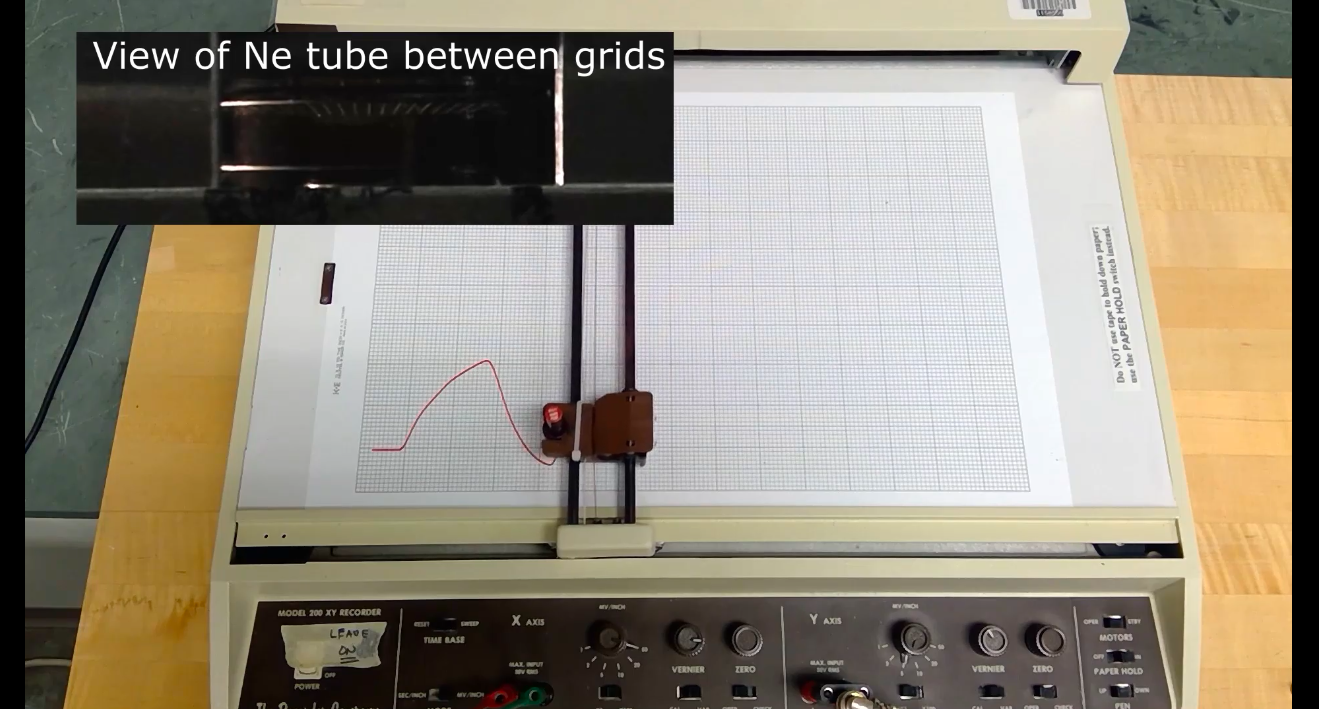
\includegraphics[width=9cm]{1st.png}
\smallskip
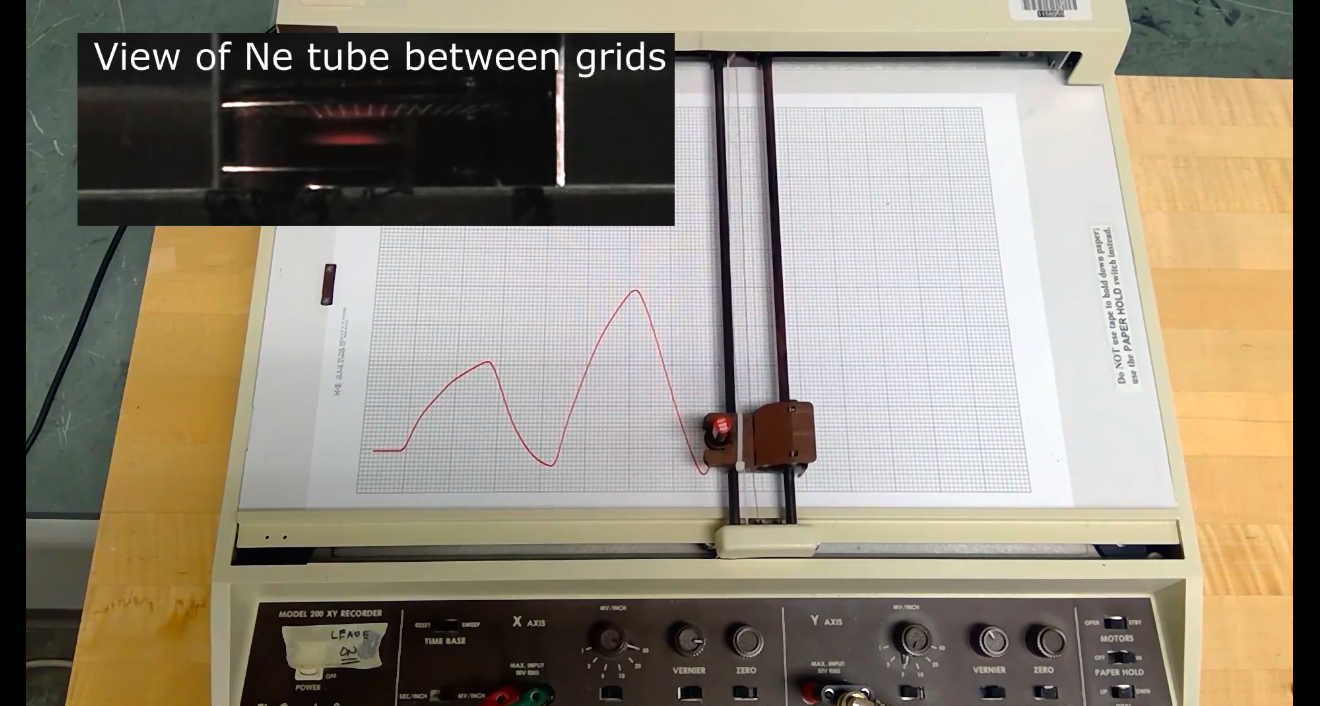
\includegraphics[width=9cm]{2nd.png}
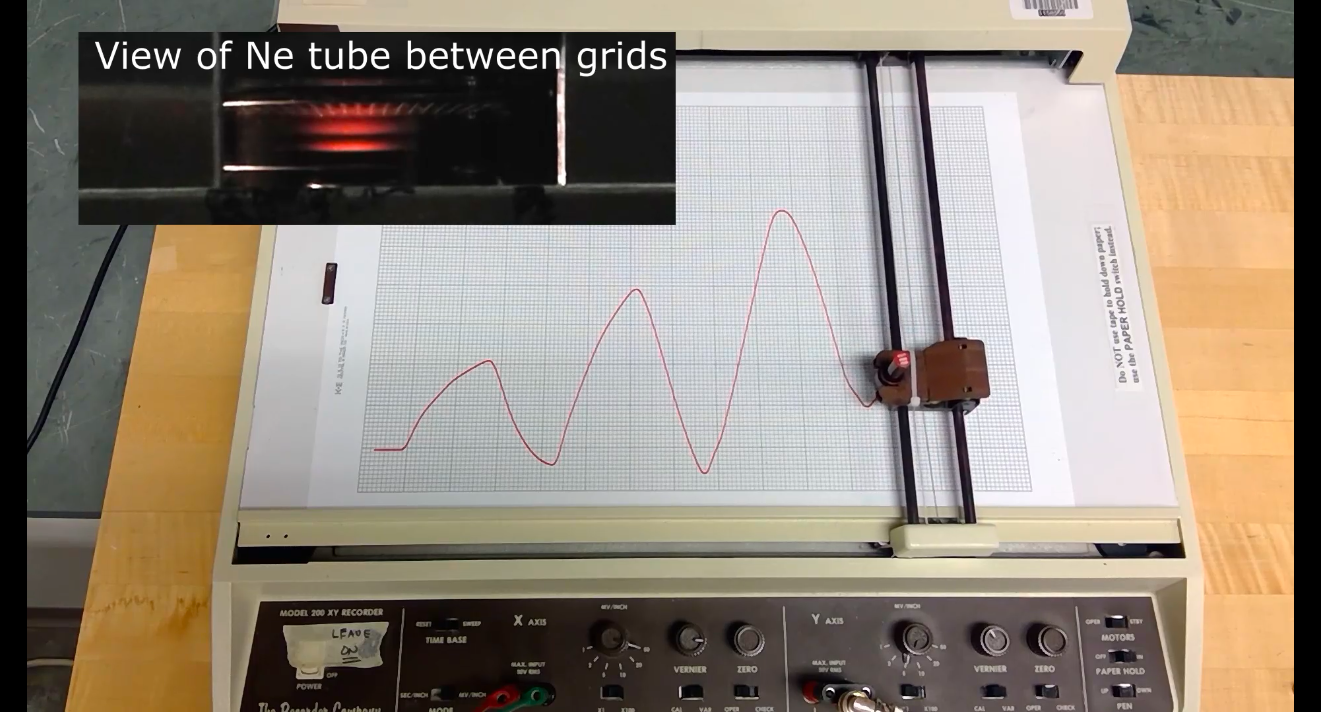
\includegraphics[width=9cm]{3rd.png}


\end{figure}

\end{document}